\documentclass{article} % For LaTeX2e
\usepackage{nips15submit_e,times}
\usepackage{hyperref}
\usepackage{url}
%\documentstyle[nips14submit_09,times,art10]{article} % For LaTeX 2.09
\usepackage{graphicx} % more modern
%\usepackage{epsfig} % less modern
%\usepackage{subfigure} 

\usepackage{amsmath}
\usepackage{amsfonts}
\usepackage{amsthm}
\usepackage{caption}
\usepackage{subcaption}

% For citations
\usepackage{natbib}

\usepackage{dsfont}

\usepackage{caption}
\DeclareCaptionType{copyrightbox}
\usepackage{subcaption}

\newcommand{\ones}{\ensuremath{\mathds{1}}}
\newcommand{\R}{\ensuremath{\mathds{R}}}
\newcommand{\veps}{\boldsymbol{\epsilon}}
\newcommand{\va}{\boldsymbol{\alpha}}
\newcommand{\Bw}{\mathbf{w}}
\newcommand{\Bx}{\mathbf{x}}
\newcommand{\By}{\mathbf{y}}
\newcommand{\Bg}{\mathbf{g}}
\newcommand{\BX}{\mathbf{X}}
\newcommand{\BK}{\mathbf{K}}
\renewcommand{\vec}[1]{\mathbf{#1}}

\newcommand{\felix}[1]{\textcolor{blue}{{\bf Felix:} #1}}
\newcommand{\niklaas}[1]{\textcolor{green}{{\bf Niklaas:} #1}}
\newcommand{\sebastian}[1]{\textcolor{red}{{\bf Sebastian:} #1}}

% For algorithms
\usepackage{algorithm}
\usepackage{algorithmic}

% As of 2011, we use the hyperref package to produce hyperlinks in the
% resulting PDF.  If this breaks your system, please commend out the
% following usepackage line and replace \usepackage{icml2016} with
% \usepackage[nohyperref]{icml2016} above.
\usepackage{hyperref}

% Packages hyperref and algorithmic misbehave sometimes.  We can fix
% this with the following command.



\title{Doubly stochastic large scale kernel learning \\ with the empirical kernel map}


\author{
Nicolaas Steenbergen\\
DFKI, Berlin, Germany\\
\texttt{nikolaas.steenbergen@dfki.de}\\
\And
Sebastian Schelter\\
TU Berlin, Berlin, Germany\\
\texttt{sebastian.schelter@tu-berlin.de}\\
\And
Felix Biessmann
TU Berlin, Berlin, Germany\\
\texttt{felix.biessmann@tu-berlin}\\
}

% The \author macro works with any number of authors. There are two commands
% used to separate the names and addresses of multiple authors: \And and \AND.
%
% Using \And between authors leaves it to \LaTeX{} to determine where to break
% the lines. Using \AND forces a linebreak at that point. So, if \LaTeX{}
% puts 3 of 4 authors names on the first line, and the last on the second
% line, try using \AND instead of \And before the third author name.

\newcommand{\fix}{\marginpar{FIX}}
\newcommand{\new}{\marginpar{NEW}}

%\nipsfinalcopy % Uncomment for camera-ready version

\begin{document}


\maketitle

\begin{abstract} 
With the rise of big data sets the popularity of kernel methods declined and deep neural network (DNNs) took over again. Most attempts to scale up kernel methods  solve the problem by simply discarding data points (or basis functions of some approximation of the kernel function). Also in many of these approaches, the main advantage of kernel methods -- modularity w.r.t. powerful kernel functions and learning methods -- is somewhat obfuscated by a significant amount of complexity of the theory or implementation details. Here we present a remarkably simple yet effective way of scaling up kernel methods via doubly stochastic optimization of the emprical kernel map, which -- to the best of our knowledge -- has not been applied to the distributed setting. We build our work on a large body of existing theoretical work on kernel machines and provide empirical evidence that the algorithm a) works in practice on large data sets b) can leverage the full power and versatility of classical kernel machines and c) is extremely simple to implement, also in distributed settings. 
\end{abstract} 


\section{Introduction\vspace{-0.1in}}
\indent When kernel methods \cite{Muller:2001p2592,learning_with_kernels,shawe2004kernel} were introduced in the machine learning community, they quickly gained popularity and became the gold standard in many applications. One reason for this was that kernel methods are powerful tools for modelling non-linear dependencies. Even more importantly, kernel methods offer a convenient split between modelling the data with an expressive set of versatile kernel functions for all kinds of data types (e.g., graph data \cite{Borgwardt:2007p13941} or text data \cite{John2000}), and the learning part, including both the learning paradigm (unsupervised vs. supervised) and the optimization. 

The main drawback of kernel methods is that one needs to compute the kernel matrix $\vec{K}\in\R^{N\times N}$, where $N$ is the number of samples. For large data sets this kernel matrix can neither be computed nor stored in memory. Even worse, the learning part of kernel machines often has complexity $\mathcal{O}(N^3)$. This renders standard formulations of kernel methods intractable for large data sets. When machine learning entered the era of web-scale data sets, artificial neural networks, enjoying learning complexities of $\mathcal{O}(N)$, took over again and have been dominating the top ranks of competitions, the press on machine learning and all major conferences since then. But the advantage of neural networks -- or other non-linear supervised algorithms that perform well on large data sets in many applications, such as Random Forests \cite{Breiman2001} -- leaves many researchers with one question (see e.g. \cite{Lu2014}): What if kernel methods could be trained on the same amounts of data that neural networks can be trained on? 

There have been several attempts to scale up kernel machines, which fall into two main categories: approximations based on subsampling of
%
\begin{itemize}
\item Fourier basis functions \cite{Rahimi2008} {\em or}
\item data points \cite{Williams2000}.
\end{itemize}
%
While both of these are powerful methods and often achieve competitive performance, most applications of these approximations solve the problem of scaling up kernel machines by discarding data points or Fourier basis functions from the computationally expensive part of the learning. Here we present a remarkably simple yet effective way of scaling up kernel methods that -- in contrast to many previous approaches -- can make use of the entire data set. 

%The method is based on well established theory on stochastic approximations \cite{sgd}. 
Similar to \cite{Dai2014}, we propose a doubly stochastic approximation to scale up kernel methods. In contrast to their work however, who use the {\em explicit} kernel map, we propose to use the empirical kernel map. While the optimization follows a similar schema, there is evidence suggesting that approximations of the explicit kernel map can result in lower performance \cite{Yang2012}.
% \felix{We will point the reader to our empirical results and some discussion in the later part of the manuscript}. 

The approach is called doubly stochastic because there are two sources of noise in the optimization: a) one samples random data points at which a noisy gradient of the dual coefficients is evaluated and b) one samples data points at which a noisy version of the empirical kernel map is evaluated. We propose a redundant data distribution scheme that allows to compute approximations that go beyond the block-diagonal of the full kernel matrix, as proposed e.g. in \cite{Deisenroth2015}. We present experiments on a single host and on a distributed infrastructure, and evaluate the algorithm on toy data and real data sets. Our results suggest that one can indeed approximate kernel methods efficiently on distributed infrastructure, thus making use of the entire data set, and obtain competitive performance. 

In the following, we give a short summary of the essentials on kernel machines, in \autoref{sec:large_scale_kernel_learning} we give a broad overview over some attempts to scale up kernel methods, \autoref{sec:dskl} outlines the main idea of the paper and \autoref{sec:experiments} contains our experiments.

\section{Kernel methods recap}\label{sec:kernels}
This section gives a short description of the essentials of kernel machines. For the sake of presentation we only consider supervised learning and assume $D$-dimensional real-valued input data $\Bx_i\in\R^D$ and a corresponding boolean label $y_i\in\{-1,1\}$. Extensions to multivariate real valued labels or unsupervised learning methods are straightforward, see  \cite{Lopez-Paz2014}. At the heart of kernel machines is the so-called {\em kernel trick}: The function $\phi^*(\Bx_i)$ to be learned, (evaluated at the $i$th data point $\Bx_i$) is modelled as a linear combination $\va\in\R^N$ of similarities between data points mapped to a (potentially infinite dimensional) {\em kernel feature space} $\mathcal{S}$

\begin{align}\label{eq:kernel_trick}
\phi^*(\Bx_i)=\sum_{j=1}^N k(\Bx_i,\Bx_j)\alpha_j
\end{align}.
Here $N$ again denotes the number of data points in a data set, $\alpha_i$ denotes the $i$th entry of $\va$, and the kernel function $k(.,.)$ measures the similarity of data points in the kernel feature space by computing inner products in $\mathcal{S}$
\begin{align}\label{eq:kernel_function}
k(\Bx_i,\Bx_j)=\langle \phi(\Bx_i), \phi(\Bx_i)\rangle_{\mathcal{S}}.
\end{align}.
%

An important requirement for kernel machines is that $\mathcal{S}$ has to have an inner product. Alternatively one can express the necessary condition as a constraint on the kernel map $k(.,.)$ 
%
\begin{align}\label{eq:kernel_condition}
\forall c\in\R: \sum_{i=1}^N \sum_{i=1}^N k(\Bx_i,\Bx_j)c_ic_j\geq 0
\end{align}
%
which is known as {\em Mercer's condition}.
Taking the shortcut through $k(.,.)$, i.e. mapping data points to $\mathcal{S}$ and computing their inner products without ever formulating the mapping $\phi$ explicitely when learning $\phi$ is sometimes called {\em kernel trick}. 

Most kernel machines then minimize a function $\mathcal{E}(y, \Bx, \va, k)$ which combines a loss function $l(y, \Bx, \va, k)$ with a regularization term $r(\va)$ that controls the complexity of $\phi$ 
%
\begin{align}\label{eq:error_function}
\mathcal{E}(y, \Bx, \va, k) = r(\va) + l(y, \Bx, \va, k).
\end{align}
%
The regularizer $r(\va)$ often takes the form of some $\mathcal{L}_p$ norm of the vector of dual coefficients $\va$, where usually $p=2$. Popular loss functions and their gradients are listed in \autoref{tab:losses}, assuming a quadratic regularizer $r(\va)=\lambda\frac{1}{2}\|\va\|_2^2$, where $\lambda$ denotes the regularization parameter.
%
\begin{table*}
\begin{center}
\begin{tabular}{ ccc } 
Algorithm & Loss $l(y, \Bx, \va, k)$ & Gradient of $\mathcal{E}$ (see \autoref{eq:error_function})\\
 \hline
Kernel SVM & $ \max \left(0,\ones-\vec{y}^{\top} \vec{K} \va \right) $& $\max \left(0,1-\left(\lambda\va_{\mathcal{I}} - \vec{y}^{\top}_{\mathcal{I}}\vec{K}_{\mathcal{I,J}}\right)\right)$\\
Kernel Ridge Regression & $ \|\vec{y} - \vec{K}\va \|_2^2 $& $\lambda\va_{\mathcal{J}} - \vec{y}_{\mathcal{J}}^{\top}\vec{K}_{\mathcal{I,J}} + \vec{K}_{\mathcal{I,J}}\vec{K}_{\mathcal{I,J}}^{\top}\va_{\mathcal{J}}$\\
%Kernel Logistic Regression & & \\
 \hline
\end{tabular}
\caption{Two examples of kernel methods with corresponding loss functions and gradients of their error functions. Note that in the proposed approach, the entire kernel matrix $\vec{K}$ is never computed; instead, one draws only a subset of indices $\mathcal{J}$ to expand the empirical kernel map and another subset of indices $\mathcal{I}$ to compute the gradient, see algorithm \autoref{alg:dskl}. \label{tab:losses}}
\end{center}
\end{table*}
%
While the examples only cover Kernel Ridge Regression, also known as Kriging \cite{kriging}, the mean function of Gaussian Processes \cite{RasWil05}, and kernel Support-Vector Machines (SVMs) \cite{Cortes1995}, other applications are relatively straightforward. We refer the interested reader to \cite{learning_with_kernels,shawe2004kernel} for a good overview of other kernel methods. 

\subsection{Large Scale Kernel Learning}\label{sec:large_scale_kernel_learning}
Evaluating the empirical kernel map in \autoref{eq:kernel_function} comes at the cost of $N$ evaluations of the kernel function, since the index $j$ (which picks the data points that are used for expanding the {\em kernel map}) runs over all data points in the data set\footnote{Actually the complexity is of $\mathcal{O}(ND)$ where $D$ is the dimensionality of the data, but as this is constant given a data set, we omit this factor here.} both for training and predicting. Computing the gradient of $\va$ on all data points requires $N$ evaluations, too, so the total complexity of computing the gradient of a kernel machine is in the order to $\mathcal{O}(N^2)$. This is the reason why kernel methods became unattractive for large data sets -- other methods like linear models or neural networks can be trained in $\mathcal{O}(N)$ time. 

We roughly categorize attempts to scale up kernel methods into two classes: a) Reducing the number of data points when evaluating the empirical kernel map in \autoref{eq:kernel_function} and b) avoiding to evaluate the empirical kernel map altogether by using an {\em explicit approximation} of the kernel map. There are more sophisticated approaches within each of these categories that can give a quite significant speedup \cite{Le2013, Rudi2015}. Here we focus on a comparison between the two approximations. We emphasize however that many of these additional improvements can also be applied to the approach proposed in this manuscript and are likely to improve convergence and runtime. In the following, we quickly summarize the major research in both categories.

\paragraph{Empirical kernel maps:} The first approach, reducing the number of data points when evaluating the kernel function, amounts to subsampling data points for computing the empirical kernel map in \autoref{eq:kernel_function}. 
The data points used to compute the empirical kernel map are sometimes referred to as {\em landmarks} \cite{Hsieh2014}. A key idea of many large scale kernel learning approaches is not to use all $N$ data points for expanding the kernel map. One line of research in this direction aims at sparsifying the vector of dual coefficients $\va$ \cite{WilsonN15, LiangP15}. 
A similar line of research follows what is commonly referred to as the {\em Nystr\"om method} \cite{Williams2000}. The idea here is that instead of using the entire kernel matrix, one can take a low-rank approximation of that matrix, computed on a randomly subsampled part of the data, in order to speed up the kernel function evaluations. There are two main problems with the above aproaches: for one, they often simply discard a large number of data points in order to do a more expensive part of the computations on a small subset of data points. Second many of these methods are tricky to implement, especially in a distributed setting. In general, applying kernel methods in distributed settings is challenging. One approach is to simply distribute the data to different workers and solve the kernel problems independently on each worker \cite{Deisenroth2015}. This implicitly assumes that the kernel matrix is a block diagonal matrix where the blocks on the diagonal are the kernels on each worker -- all the rest of the kernel matrix is neglected.

\paragraph{Explicit kernel maps:} Recent approaches for large scale kernel learning avoid computation of the kernel matrix by relying on {\em explicit} forms of the kernel function \cite{Rahimi2008,Vedaldi2010}. The basic idea is that instead of using a kernel function $k$, which {\em implicitly} projects the data to kernel feature space $\mathcal{S}$ and computes the inner products in that space in one step, {\em explicit} kernel functions just perform the first step, mapping to kernel feature space with an approximation of the kernel map $\phi(.)$. This has the advantage that the effective number of features can be controlled directly. The model then learns simply a linear combination of these features. Explicit feature maps often express the kernel function as a set of Fourier basis functions. An excellent and comprehensive overview of kernel functions and their explicit representations can be found in \cite{Dai2014}. A more detailed explanation with graphical illustrations for a small set of kernel functions can be found in \cite{Vedaldi2010}. In the context of large-scale kernel learning this method was popularized by Rahimi and Recht under the name of {\em random kitchen sinks} \cite{Rahimi2008}. 

\paragraph{Which approximation is better?}
Both approaches, {\em implicit kernel maps} and {\em explicit kernel maps}, are similar in that they approximate a potentially infinite dimensional space $\mathcal{S}$. The main difference is that for empirical kernel map approaches, the approximation samples data points (and in most cases simply {\em discards} a lot of data points), while in the case of explicit kernel map approximations the approximation samples random Fourier basis functions. In practice there are many limitations on how much data can be acquired and how much data can be processed efficiently. The type of data can also make a difference in the performance of either approximation: When using the empirical kernel map on extremely sparse data, the empirical kernel function evaluated on a small subset of data points will return 0 in most cases -- while Fourier bases with low frequencies will cover the space of the data much better. 

We hypothesize that the question which of these approximations is better in practice is probably best answered with: It depends - mostly on the data. 
Some empirical evidence suggests that the Nystr\"om approximation is better than random kitchen sinks \cite{Yang2012}. The authors of \cite{Vedaldi2010} perform an excellent comparison of various explicit kernel map approximations and empirical kernel maps and highlight some of the advantages in the empirical kernel map approach: Empirical kernel maps can model some parts of the input distribution better -- but they have to be trained on data; this can be considered as a disadvantage. But then again any machine learning algorithm has to learn from data and there could be scenarios in which learning the feature representation (via empirical kernel maps) along the way can give some performance gains. Taken together we are not aware of a concise comparison of the two approaches in a distributed setting. In our experimental section we aim at a first direct comparison between the two, keeping the optimization part fix and concentrating on the type of approximation. 
%
\section{Doubly stochastic kernel learning}\label{sec:dskl}
This section describes the learning approach, which follows the pseudocode sketched in Algorithm \autoref{alg:dskl} for a pair of data points. The idea is that in each iteration a random sample $\mathcal{I}\subseteq\{1,2,\dots,N\}, |\mathcal{I}|=I$ of data points is chosen for computing the gradient of the dual coefficients $\va$ and another (independent) random sample  $\mathcal{J}\subseteq\{1,2,\dots,N\}, |\mathcal{J}|=J$ of data points is chosen for expanding the empirical kernel map $k(.,.)$. Note that this is very similar to Algorithm 1 and 2 in \cite{Dai2014}, except that instead of drawing random basis functions of the kernel function approximation, we sample random data points. If one were to compute the entire kernel matrix $\vec{K}\in\R^{N\times N}$, this procedure would correspond to sampling a rectangular submatrix $\vec{K}_{\mathcal{I,J}}\in\R^{I\times J}$. The number of data points sampled for expanding the empirical kernel map as well as the number of data points to compute the gradient are important parameters that determine the noise of the gradient of the dual coefficients and the noise if the empirical kernel map, respectively. The pseudocode in algorithm \autoref{alg:dskl} summarises the entire procedure, which alternates two steps: 1) sample a random submatrix of the kernel matrix and 2) take a gradient step along the direction of $\frac{\partial\mathcal{E}}{\partial \va_{\mathcal{J}}}$.

% 
\begin{algorithm}
  \begin{algorithmic}
    \caption{Doubly Stochastic Kernel Learning\label{alg:dskl}}
     \REQUIRE $(\Bx_i,y_i),i\in\{1,\dots,N\},\Bx_i\in\R^{D},~y_i\in\{-1,+1\}$, Kernel $k(.,.)$
    \ENSURE Dual coefficients $\va$ 
   \STATE \# Initialize coefficients $\va$, initialize counter $i=0$
   \WHILE{Not Converged}
   \STATE $t\gets t+1$
   \STATE \# Sample indices $\mathcal{I}$ for gradient 
   \STATE $\mathcal{I}\sim\text{unif}(1,N)$
   \STATE \# Sample indices $\mathcal{J}$ for empirical kernel map
   \STATE $\mathcal{J}\sim\text{unif}(1,N)$
   \STATE \# Compute Gradient
   \STATE $\vec{g}_{\mathcal{J}} \gets \frac{\partial \mathcal{E}}{\partial\va_{\mathcal{J}}}$ (see \autoref{tab:losses})
   \STATE \# Update weight vector 
   \STATE $\forall j\in\mathcal{J}: \alpha_j\gets\alpha_j - 1/t~ g_j$ 
   \ENDWHILE
  \end{algorithmic}
\end{algorithm}
%
Note that in contrast to many other kernel approximations the memory footprint of this algorithm is low: While low-rank approximations need to store the low rank factors, algorithm \autoref{alg:dskl} requires only to store the dual coefficients $\va$. 
The learning rate parameter here is simply set to $1/t$ where $t$ is the number of iterations. It is good practice to adjust that parameter according to some more sophisticated schedule. Moreover, as the method is perfoming stochastic gradient descent on the dual coefficients of the kernel map, all standard methods to speed up convergence can in principle be applied. Also special care has to be taken when running the algorithm in a distributed fashion. However we emphasize that the complexity of the implementation remains essentially the same when running this algorithm on distributed infrastructure, as explained in more detail in \autoref{sec:distributed}.
%
\section{Experiments}
This experimental section will describe some experiments on artificially generated toy data and on publicly available real-world data sets. All experiments will use a support-vector machine with RBF kernel, for the sake of comparability. We performed experiments on a single host as well as on distributed infrastructure. Most comparisons with other algorithms, in particular with batch SVMs, were done on a single host. We used the batch SVM implementation available in scikit learn \cite{sklearn_api}. For all models we tunes hyperparameters with two-fold cross-validation and exhaustive gridsearch; reported accuracies were computed on a held out test set of the same size as the training set. For batch and SGD algorithms the hyperparameters were the regularization parameter and RBF scale, both were optimized on a logarithmic grid from $10^{-6}-10^6$; additional parameters for the SGD approaches were the stepsize (candidates were $10^{-4}-10^4$), the minibatch size for computing the gradient $I$ and for doubly stochastic kernel learning and for random fourier features also the number of kernel expansion coefficients $J$ or random fourier features, respectively. Both were set to 100, sampling of $\mathcal{I,J}$ was done with replacement and we ran 100 gradient steps for all algorithms trained with SGD. More iterations improved the results in the cases we tested, but as the gridsearch was time consuming and the point of the comparisons is that the proposed method achieves comparable performance, we decided to use only 100 iterations. 

\subsection{Comparisons with related methods}
We compared the proposed method with other kernel approximations as well as with batch kernel SVMs . Comparisons were done with random kitchen sinks (RKS) where the number of basis functions matches the number of expansion coefficients $J$. In order to compare with standard large-scale kernel approximations that use only a subset of data points we also compare with a version in which we first draw one random sample from the data and train the algorithm with that subset only. While most of these methods that use just a subset of the data use much more sophisticated schemes for selecting that subset and smarter ways of extrapolating, we wanted to focus on the main differences here, which is training on a fix random subset of the data. 

\subsection{Single host experiments}\label{sec:single_host}
We generated toy data from an XOR problem as shown in \autoref{fig:toy_data}. Data from one class (yellow dots) is drawn from a spherical gaussian distribution $\mathcal{N}(0,0.2)$ around $[1,1]^\top$ and $[-1,-1]^\top$ and data points from the other class (red dots) were drawn from the same gaussian distribution centered around $[1,-1]^\top$ and $[-1,1]^\top$. 
%
\begin{figure}[!ht]
    \centering
        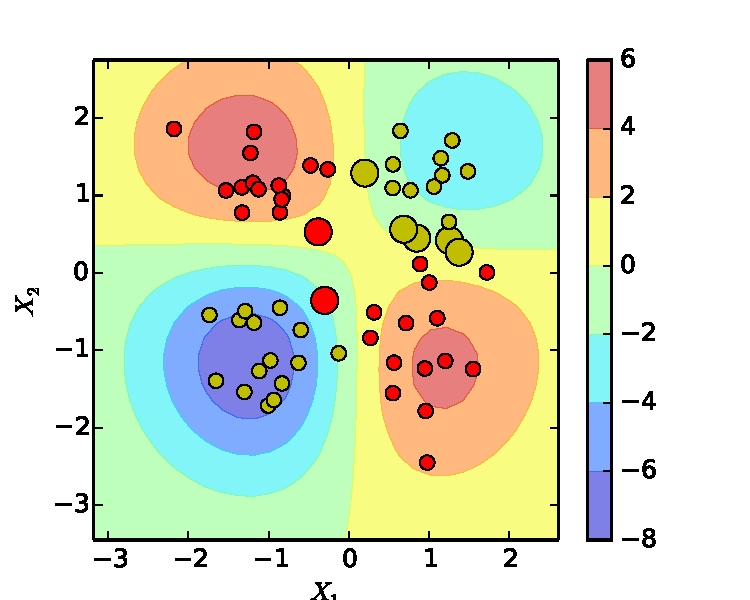
\includegraphics[width=0.4\columnwidth]{imgs/svm_kernel}
        \caption{
        The XOR problem, a two class nonlinear prediction problem. Background colors show the classification hyperplane learned by doubly stochastic SVM learning; support vectors are shown as larger circles.}
        \label{fig:toy_data}
\end{figure}
%
\autoref{fig:toydata_comparisons} shows comparisons of the proposed method with other, related approaches, as well as with a batch setting. 
The error on the test set when varying $I$, the number of samples for computing the gradient, is plotted in \autoref{fig:expand_20_pred_1} and \autoref{fig:expand_20_pred_50}. The error when varying $J$, the number of expansion coefficients is shown in \autoref{fig:pred_20_expand_1} \autoref{fig:pred_20_expand_50}. Note that with too few data points for computing the gradient or the expansion, both random kitchen sinks as well as a fix sample of data points have an advantage over the doubly stochastic approach. When as the number of data points in the gradient computation and the kernel map expansion increases however, doubly stochastic kernel learning achieves performances comparable to batch methods (indicated as dotted line).
%
\begin{figure}[!ht]
   \centering
    \begin{subfigure}[b]{0.235\textwidth}
        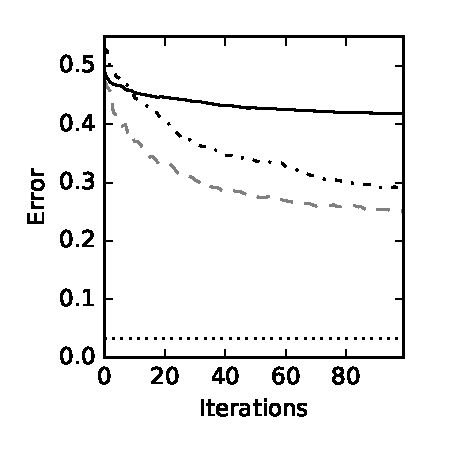
\includegraphics[width=\textwidth]{imgs/rks_emp_comparison-expand-20-pred-1}
        \caption{$I=1, J=20$}
        \label{fig:expand_20_pred_1}
    \end{subfigure}
    \hfill
    \begin{subfigure}[b]{0.235\textwidth}
        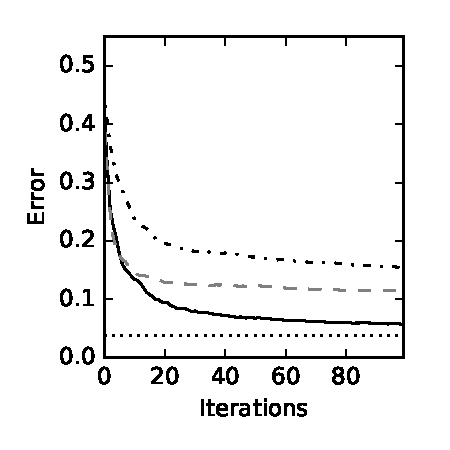
\includegraphics[width=\textwidth]{imgs/rks_emp_comparison-expand-20-pred-50}
        \caption{$I=50, J=20$}
        \label{fig:expand_20_pred_50}
    \end{subfigure}\\
        \begin{subfigure}[b]{0.235\textwidth}
        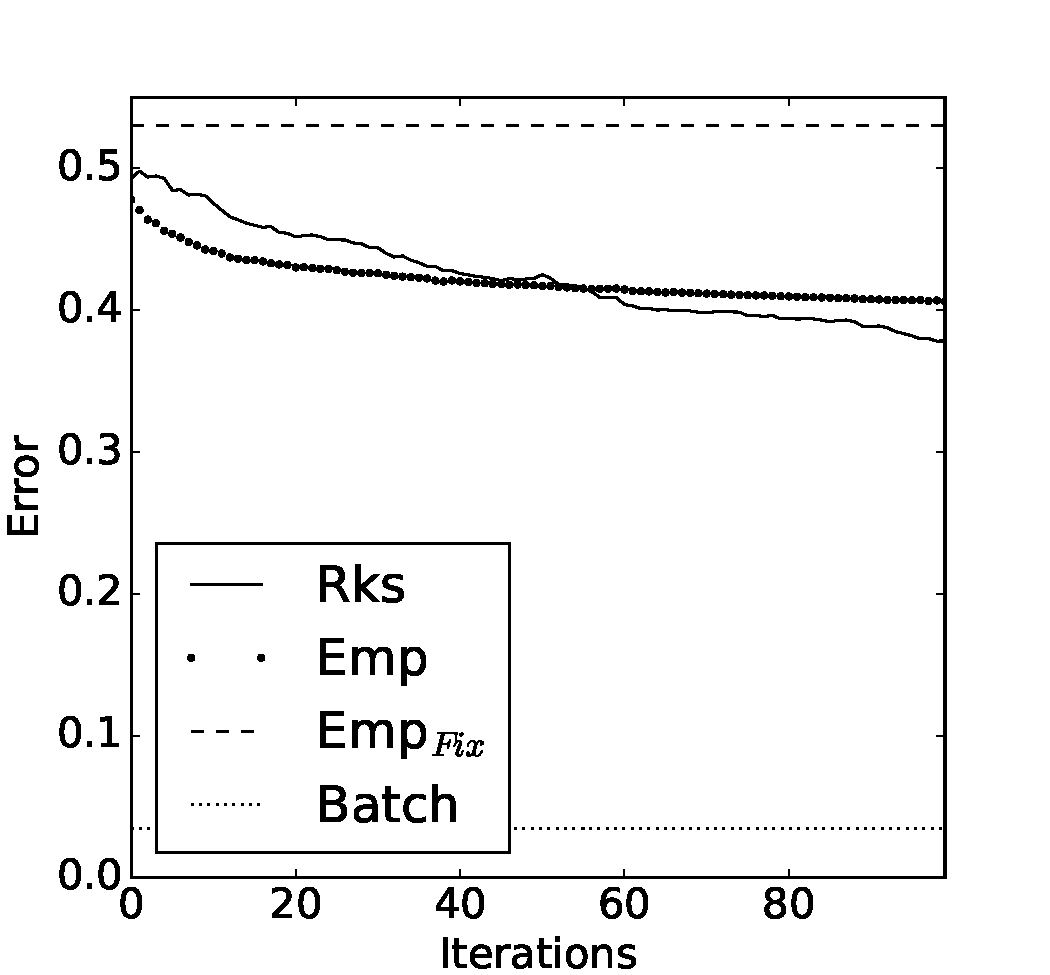
\includegraphics[width=\textwidth]{imgs/rks_emp_comparison-pred-20-expand-1}
        \caption{$I=20, J=1$}
        \label{fig:pred_20_expand_1}
    \end{subfigure}
    \hfill
    \begin{subfigure}[b]{0.235\textwidth}
        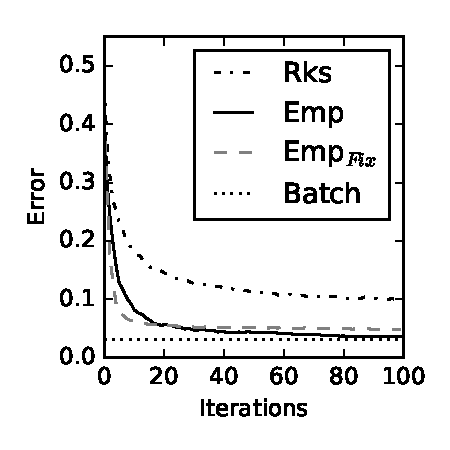
\includegraphics[width=\textwidth]{imgs/rks_emp_comparison-pred-20-expand-50}
        \caption{$I=20, J=50$}
        \label{fig:pred_20_expand_50}
    \end{subfigure}
    \caption{Error on test data for XOR problem in \autoref{fig:toy_data} for doubly stochastic kernel learning with the empirical kernel map (Emp), random kitchen sinks (RKS), random subsampling (Emp$_{\text{Fix}}$) and batch SVM}
    \label{fig:toydata_comparisons}
\end{figure}
%
We performed experiments on a number of standard benchmark real world data sets available on the libsvm homepage\footnote{\url{https://www.csie.ntu.edu.tw/~cjlin/libsvmtools/datasets/binary.html}}. In order to be able to run the batch comparisons, these comparisons are run on a single host and small data sets. Large scale experiments are discussed in \autoref{sec:distributed}. For all experiments we sampled $\min(1000,N_{\text{dataset}})$ data points where $N_{\text{dataset}}$ is the number of data points in that data set and took half the data for training and half the data for testing, including hyperparameter optimization on the training set. We ran 10 repetitions of each experiment and show the test set error in \autoref{tab:small_realdata}. In all data sets we have looked at, the proposed doubly stochastic empirical kernel learning approach achieves errors comparable to that of a batch SVM. In some cases the batch SVM achieves perfect accuracy and DSEKL still results in a few errors, we emphasize however that these comparisons are done to show that DSEKL can achieve performances comparable with batch methods. Refining the SGD optimization or running more iterations would have probably further improved the performance. We did not do that as we merely wanted to show a proof of concept. Also note that the proposed DSEKL approach uses only a fraction of the data in each step. This allows training on much larger data sets, which will be discussed in the next section.
%
\begin{table}
\begin{center}
\begin{tabular}{ ccc } 
Data Set & DSEKL & Batch\\
 \hline
MNIST small & 0.00$\pm$0.01  & 0.00$\pm$0.01\\
Diabetes & 0.20$\pm$0.02  & 0.22$\pm$0.02\\
Breast Cancer &  0.03$\pm$0.01 & 0.03$\pm$0.01\\
Mushrooms & 0.03$\pm$0.01 & 0.00$\pm$0.00\\
Sonar & 0.22$\pm$0.07 & 0.26$\pm$0.04\\
Skin/non-skin & 0.03$\pm$0.01 &  0.01$\pm$0.00\\
Madelon & 0.03$\pm$0.01 &  0.00$\pm$0.00\\
 \hline
\end{tabular}
\caption{Test error (mean $\pm$ standard deviation across 10 repetitions) on real world data sets. Doubly stochastic empirical kernel learning (DSEKL) achieves performances comparable to batch kernel SVM. \label{tab:small_realdata}}
\end{center}
\end{table}
%
\subsection{Distributed infrastructure}\label{sec:distributed}
This section describes the experiments performed on distributed infrastructure. We list the pseudocode in algorithm\autoref{alg:dskl_svm_distributed}. The only difference to algorithm \autoref{alg:dskl} is that the data is distributed to multiple workers in a cluster and the learning happens in parallel. We use sampling with replacement to re-partition the data onto the different workers. Partition sizes can be chosen flexibly which ensures that we have redundancy in the data partitions, i.e. one data point can be on multiple machines. This allows the algorithm to access more than just the block-diagonal parts of the full kernel matrix, as opposed to approaches such as \cite{Deisenroth2015}. 

As a real-world data set we use a larger version of the MNIST data set, see e.g. \url{http://leon.bottou.org/projects/infimnist}, for the sake of easier comparison with other studies \cite{Lu2014, Dai2014}.

\begin{algorithm}
  \begin{algorithmic}[1]
    \caption{Distributed Non-Linear Support-Vector Machine\label{alg:dskl_svm_distributed}}
      \REQUIRE sample size $s$, number of workers $K$
   \STATE \# Initialize coefficients $\va$
      \STATE \# Generate samples for all workers
      \STATE $\vec{X}^{(0)},\dots,\vec{X}^{(K)} \leftarrow$ samples of size $s$ from $\vec{X}$
      \STATE $\vec{y}^{(0)},\dots,\vec{y}^{(K)} \leftarrow$ corresponding label samples of $\vec{y}$
      \STATE $\vec{G} \leftarrow \mathbb{I}$
      \WHILE{Not Converged}
      	    \STATE \# Broadcast $\va$ to all workers
	    \FORALL{workers $k$}      
		\STATE $\hat{\vec{G}}^{(k)} \leftarrow \mathbf{0}$
		\STATE \# Sample indices $\mathcal{I}^{(k)}$ for gradient 
		\STATE \# Sample indices $\mathcal{J}^{(k)}$ for empirical kernel map
		\STATE \# Compute gradients as in Algorithm~\autoref{alg:dskl}
		\STATE $\vec{g}^{(k)} \gets \frac{\partial \mathcal{E}}{\partial\va^{(k)}}$ (see \autoref{tab:losses})
		\STATE $\hat{G}_{ii}^{(k)} \leftarrow \left(g^{(k)}_{ji}\right)^2$ for all $i \in\mathcal{I}^{(k)}$ and $j\in\mathcal{J}^{(k)}$
	    \ENDFOR
	\STATE \# Aggregate inverse gradients for dampening updates of $\va$
        	\STATE $\vec{G} \leftarrow \vec{G} + \sum_k \hat{\vec{G}}^{(k)}$     
	\STATE \# Update weight vector 
        \STATE $\va \leftarrow \va - G^{-\frac{1}{2}} \sum_k \vec{g}^{(k)}$
      \ENDWHILE
  \end{algorithmic}
\end{algorithm}

We follow a very simple scheme for the distributed implementation in which we draw a large set of samples with replacement in the beginning when partitioning the data onto the different workers. This redundant sample is then cached on the workers, instead of resampling in every iteration and re-partitioning the data. The rationale is to bring the computation as close as possible to the data and reduce communication cost. The simplicity of the distributed algorithm allows it to be easily implemented in most distributed data processing systems currently deployed in industry, such as \textit{Apache Spark}~\cite{Zaharia2012}, \textit{Apache Flink}~\cite{Alexandrov2014} or \textit{h20}\footnote{http://www.h2o.ai/}. 

We create a reference implementation in Spark as follows. Here the execution is controlled by a driver program on a master machine which schedules the computations on the workers in the cluster. First, we generate the indexes for the partition samples in a multithreaded fashion on the driver machine~(c.f., lines 3 \& 4). Next, we execute a distributed broadcast-join between the generated indexes and the datapoints. We group the join result by the partition indexes and pack all datapoints $\vec{X}^{(k)}$ and $\vec{y}^{(k)}$ of a partition $k$ into a memory-efficient datastructure. We advise the system to cache the partitions in the main memory of the cluster. Precomputing the partitions in this way allows us to execute the actual learning algorithm via a simple iterative \textit{Map-Reduce-Update} scheme. We initialize the vector of dual coefficients $\alpha$ and broadcast it to all worker machines. Then, we execute a single iteration of the learning algorithm as follows. First, we run the gradient computation~(c.f., lines 9 \& 14) in an embarassingly parallel manner on every partition via a \textit{map} operation. The summations of the gradients and their inverses (in lines 17 \& 19) require a global aggregation, which we conduct via a global \textit{reduce}, executed in a tree aggregation. Finally, we \textit{update} the coefficients vector (in line 19) and re-broadcast it to all workers. 

\begin{figure}[!ht]
  \centering
    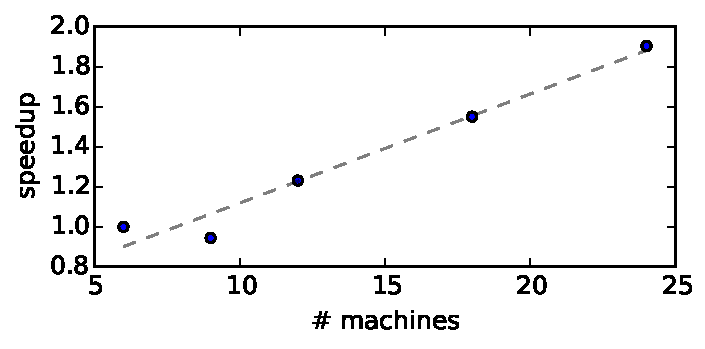
\includegraphics[width=0.6\columnwidth]{imgs/linear-speedup}
     \caption{Linear speedup when increasing computing resources.}
  \label{fig:scalability}
\end{figure}

We first run a scale-out experiment to determine how our implementation scales with increasing cluster resources. We use the \textit{mnist8m} dataset with 8 million observations, consisting of 784 features each, giving us a matrix with more than $6$ billion cells as input data. We run our spark implementation of Algorithm~\ref{alg:dskl_svm_distributed} on this dataset on a cluster comprised of 24 machines and choose the sample sizes in a way that the aggregate sample size amounts to the full dataset. We start by leveraging 6 machines and subsequently increase this number to 9, 12, 18 and the full 24 machines. We measure the runtime for each subsequent run; On the full cluster, an iteration takes approximately 6 seconds\footnote{note that our implementation is a proof of concept in Scala; there is much rooom for performance improvements by using a language like C++ and native matrix libraries; furthermore, the runtime is dependent on the number of samples drawn}; We compute the speedups in comparison to the smallest setup (c.f.,~Figure~\ref{fig:scalability}) and find that increasing the cluster resources results in a roughly linear speedup. Although the speedups are far from perfect, mostly due to the costly broadcast operation, our algorithm shows the desired scalability property: the ability to handle more data by simply increasing cluster resources.

\section{Conclusion}
When modelling complex functions, the practitioner usually has three main options: Decision-Tree based methods, Neural Networks and Kernel methods. While Tree based methods appear to dominate most Kaggle competitions and in general have a stunning performance on real-world data sets \cite{Caruana2006}. The results of this paper were purely empirical and could also be interpreted as: Tree-based implementations work best out-of-the-box. Implementing such a method however can be difficult, especially in a distributed setting. More importantly tree based methods are mostly known for supervised learning tasks -- unsupervised modelling with tree-based methods appears to be not a well established genre. Neural Networks became extremely popular and powerful tools, mostly due to the availability of novel technology for training them. This technology is of course beneficial for all other learning paradigms as well. The results obtained with the above models are however difficult to compare with kernel methods: Kernel methods do not scale to the amounts of data used to achieve state of the art performance with deep networks. And it is difficult to compare methods if they were not trained on the same amount of data.

%From a theoretical standpoint one could argue that there is not much reason to believe why kernel methods should be superior or inferior to neural networks; following the universal approximation theorem  \cite{Cybenko1989}, any function can be approximated with a single hidden layer. And even many introductory tutorials to neural networks highlight the commonalities between these shallow neural networks and kernel machines. 

Deep neural networks yield stunning performance improvements on many tasks -- but they can be tricky to design and train.
This is where kernel methods can offer some advantages: Instead of designing a complicated network architecture one can simply pick an off-the-shelf kernel function for a given type of data and then do model selection over just a handful of kernel parameters. And instead of tweaking a tree-based algorithm or a neural network into an unsupervised learning paradigm, one can combine a kernel function with both unsupervised {\em and} supervised learning in a principled way.  

Many researchers have argued before that when properly applied to large data sets kernel methods can be a sensible alternative to other methods \cite{Lu2014}. Here we extend the set of large scale kernel methods by a very simple algorithm that is easy to implement and distribute and achieves competitive performance. 
\felix{We will also discuss how it depends on the data set whether it is better in practice to either randomly sample basis functions of explicit kernel functions approximations or data points for expansion of the empirical kernel function. }

\newpage

\bibliography{dskl}
\bibliographystyle{plain}

\end{document} 
